\documentclass{ctexart}
    \usepackage{enumitem}
    \usepackage{graphicx}
\begin{document}
    \title{汉明码上机实验}
    \author{赵丰}
    \maketitle
    \begin{enumerate}[label = (\alph*)]
    \item display 第一个窗口显示 BSC信道的 error vector 数据, 第二个窗口显示用 Hamming 编码后出错的数据。
    \item 将 BSC 信道的 error rate 调大后误码率变大。
    \item 
    
    \begin{figure}[!ht]
        \centering
        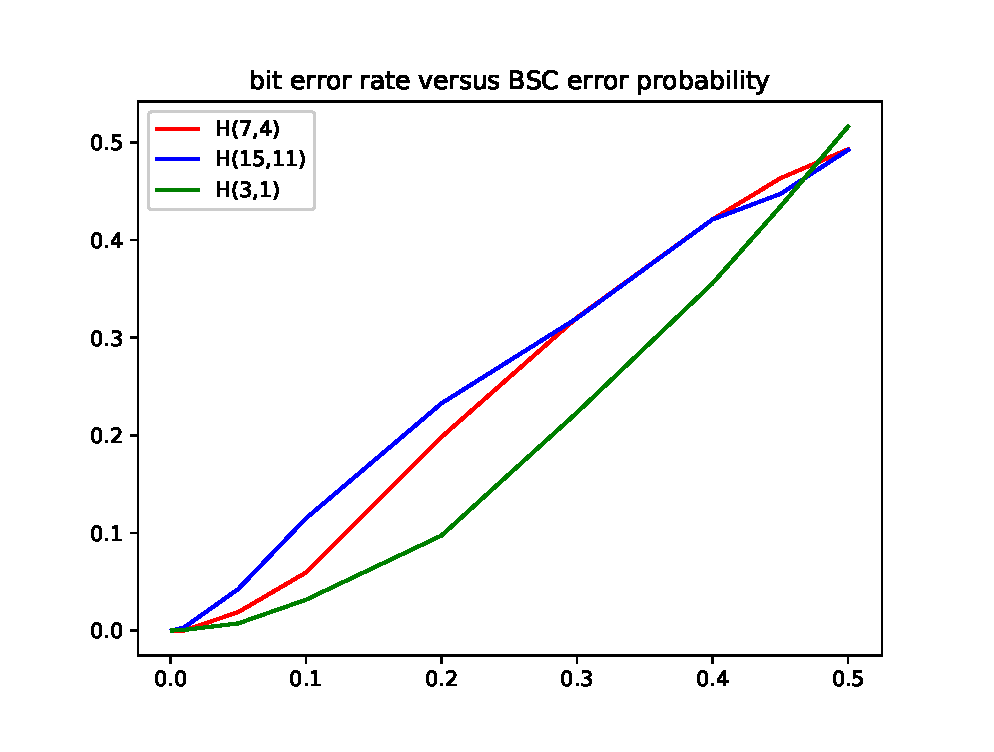
\includegraphics[width=7cm]{hamming.eps}
        \caption{不同汉明码误码率比较}\label{fig}
    \end{figure}

    \item 从图~\ref{fig} 可见, 码长较短的汉明码误码率低、纠错性能好, 但码率也低, 冗余较大。
    \end{enumerate}
\end{document}